% Options for packages loaded elsewhere
\PassOptionsToPackage{unicode}{hyperref}
\PassOptionsToPackage{hyphens}{url}
\PassOptionsToPackage{dvipsnames,svgnames,x11names}{xcolor}
%
\documentclass[
  letterpaper,
  DIV=11,
  numbers=noendperiod]{scrartcl}

\usepackage{amsmath,amssymb}
\usepackage{iftex}
\ifPDFTeX
  \usepackage[T1]{fontenc}
  \usepackage[utf8]{inputenc}
  \usepackage{textcomp} % provide euro and other symbols
\else % if luatex or xetex
  \usepackage{unicode-math}
  \defaultfontfeatures{Scale=MatchLowercase}
  \defaultfontfeatures[\rmfamily]{Ligatures=TeX,Scale=1}
\fi
\usepackage{lmodern}
\ifPDFTeX\else  
    % xetex/luatex font selection
\fi
% Use upquote if available, for straight quotes in verbatim environments
\IfFileExists{upquote.sty}{\usepackage{upquote}}{}
\IfFileExists{microtype.sty}{% use microtype if available
  \usepackage[]{microtype}
  \UseMicrotypeSet[protrusion]{basicmath} % disable protrusion for tt fonts
}{}
\makeatletter
\@ifundefined{KOMAClassName}{% if non-KOMA class
  \IfFileExists{parskip.sty}{%
    \usepackage{parskip}
  }{% else
    \setlength{\parindent}{0pt}
    \setlength{\parskip}{6pt plus 2pt minus 1pt}}
}{% if KOMA class
  \KOMAoptions{parskip=half}}
\makeatother
\usepackage{xcolor}
\setlength{\emergencystretch}{3em} % prevent overfull lines
\setcounter{secnumdepth}{5}
% Make \paragraph and \subparagraph free-standing
\ifx\paragraph\undefined\else
  \let\oldparagraph\paragraph
  \renewcommand{\paragraph}[1]{\oldparagraph{#1}\mbox{}}
\fi
\ifx\subparagraph\undefined\else
  \let\oldsubparagraph\subparagraph
  \renewcommand{\subparagraph}[1]{\oldsubparagraph{#1}\mbox{}}
\fi

\usepackage{color}
\usepackage{fancyvrb}
\newcommand{\VerbBar}{|}
\newcommand{\VERB}{\Verb[commandchars=\\\{\}]}
\DefineVerbatimEnvironment{Highlighting}{Verbatim}{commandchars=\\\{\}}
% Add ',fontsize=\small' for more characters per line
\usepackage{framed}
\definecolor{shadecolor}{RGB}{241,243,245}
\newenvironment{Shaded}{\begin{snugshade}}{\end{snugshade}}
\newcommand{\AlertTok}[1]{\textcolor[rgb]{0.68,0.00,0.00}{#1}}
\newcommand{\AnnotationTok}[1]{\textcolor[rgb]{0.37,0.37,0.37}{#1}}
\newcommand{\AttributeTok}[1]{\textcolor[rgb]{0.40,0.45,0.13}{#1}}
\newcommand{\BaseNTok}[1]{\textcolor[rgb]{0.68,0.00,0.00}{#1}}
\newcommand{\BuiltInTok}[1]{\textcolor[rgb]{0.00,0.23,0.31}{#1}}
\newcommand{\CharTok}[1]{\textcolor[rgb]{0.13,0.47,0.30}{#1}}
\newcommand{\CommentTok}[1]{\textcolor[rgb]{0.37,0.37,0.37}{#1}}
\newcommand{\CommentVarTok}[1]{\textcolor[rgb]{0.37,0.37,0.37}{\textit{#1}}}
\newcommand{\ConstantTok}[1]{\textcolor[rgb]{0.56,0.35,0.01}{#1}}
\newcommand{\ControlFlowTok}[1]{\textcolor[rgb]{0.00,0.23,0.31}{#1}}
\newcommand{\DataTypeTok}[1]{\textcolor[rgb]{0.68,0.00,0.00}{#1}}
\newcommand{\DecValTok}[1]{\textcolor[rgb]{0.68,0.00,0.00}{#1}}
\newcommand{\DocumentationTok}[1]{\textcolor[rgb]{0.37,0.37,0.37}{\textit{#1}}}
\newcommand{\ErrorTok}[1]{\textcolor[rgb]{0.68,0.00,0.00}{#1}}
\newcommand{\ExtensionTok}[1]{\textcolor[rgb]{0.00,0.23,0.31}{#1}}
\newcommand{\FloatTok}[1]{\textcolor[rgb]{0.68,0.00,0.00}{#1}}
\newcommand{\FunctionTok}[1]{\textcolor[rgb]{0.28,0.35,0.67}{#1}}
\newcommand{\ImportTok}[1]{\textcolor[rgb]{0.00,0.46,0.62}{#1}}
\newcommand{\InformationTok}[1]{\textcolor[rgb]{0.37,0.37,0.37}{#1}}
\newcommand{\KeywordTok}[1]{\textcolor[rgb]{0.00,0.23,0.31}{#1}}
\newcommand{\NormalTok}[1]{\textcolor[rgb]{0.00,0.23,0.31}{#1}}
\newcommand{\OperatorTok}[1]{\textcolor[rgb]{0.37,0.37,0.37}{#1}}
\newcommand{\OtherTok}[1]{\textcolor[rgb]{0.00,0.23,0.31}{#1}}
\newcommand{\PreprocessorTok}[1]{\textcolor[rgb]{0.68,0.00,0.00}{#1}}
\newcommand{\RegionMarkerTok}[1]{\textcolor[rgb]{0.00,0.23,0.31}{#1}}
\newcommand{\SpecialCharTok}[1]{\textcolor[rgb]{0.37,0.37,0.37}{#1}}
\newcommand{\SpecialStringTok}[1]{\textcolor[rgb]{0.13,0.47,0.30}{#1}}
\newcommand{\StringTok}[1]{\textcolor[rgb]{0.13,0.47,0.30}{#1}}
\newcommand{\VariableTok}[1]{\textcolor[rgb]{0.07,0.07,0.07}{#1}}
\newcommand{\VerbatimStringTok}[1]{\textcolor[rgb]{0.13,0.47,0.30}{#1}}
\newcommand{\WarningTok}[1]{\textcolor[rgb]{0.37,0.37,0.37}{\textit{#1}}}

\providecommand{\tightlist}{%
  \setlength{\itemsep}{0pt}\setlength{\parskip}{0pt}}\usepackage{longtable,booktabs,array}
\usepackage{calc} % for calculating minipage widths
% Correct order of tables after \paragraph or \subparagraph
\usepackage{etoolbox}
\makeatletter
\patchcmd\longtable{\par}{\if@noskipsec\mbox{}\fi\par}{}{}
\makeatother
% Allow footnotes in longtable head/foot
\IfFileExists{footnotehyper.sty}{\usepackage{footnotehyper}}{\usepackage{footnote}}
\makesavenoteenv{longtable}
\usepackage{graphicx}
\makeatletter
\def\maxwidth{\ifdim\Gin@nat@width>\linewidth\linewidth\else\Gin@nat@width\fi}
\def\maxheight{\ifdim\Gin@nat@height>\textheight\textheight\else\Gin@nat@height\fi}
\makeatother
% Scale images if necessary, so that they will not overflow the page
% margins by default, and it is still possible to overwrite the defaults
% using explicit options in \includegraphics[width, height, ...]{}
\setkeys{Gin}{width=\maxwidth,height=\maxheight,keepaspectratio}
% Set default figure placement to htbp
\makeatletter
\def\fps@figure{htbp}
\makeatother

% load packages
\usepackage{geometry}
\usepackage{xcolor}
\usepackage{eso-pic}
\usepackage{fancyhdr}
\usepackage{sectsty}
\usepackage{fontspec}
\usepackage{titlesec}

%% Set page size with a wider right margin
\geometry{a4paper, total={170mm,257mm}, left=20mm, top=20mm, bottom=20mm, right=50mm}

%% Let's define some colours
\definecolor{light}{HTML}{E6E6FA}
\definecolor{highlight}{HTML}{800080}
\definecolor{dark}{HTML}{330033}

%% Let's add the border on the right hand side 
\AddToShipoutPicture{% 
    \AtPageLowerLeft{% 
        \put(\LenToUnit{\dimexpr\paperwidth-3cm},0){% 
            \color{light}\rule{3cm}{\LenToUnit\paperheight}%
          }%
     }%
     % logo
    \AtPageLowerLeft{% start the bar at the bottom right of the page
        \put(\LenToUnit{\dimexpr\paperwidth-2.25cm},27.2cm){% move it to the top right
            \color{light}
\includegraphics[width=1.5cm]{_extensions/nrennie/PrettyPDF/logo.png}
          }%
     }%
}

%% Style the page number
\fancypagestyle{mystyle}{
  \fancyhf{}
  \renewcommand\headrulewidth{0pt}
  \fancyfoot[R]{\thepage}
  \fancyfootoffset{3.5cm}
}
\setlength{\footskip}{20pt}

%% style the chapter/section fonts
\chapterfont{\color{dark}\fontsize{20}{16.8}\selectfont}
\sectionfont{\color{dark}\fontsize{20}{16.8}\selectfont}
\subsectionfont{\color{dark}\fontsize{14}{16.8}\selectfont}
\titleformat{\subsection}
  {\sffamily\Large\bfseries}{\thesection}{1em}{}[{\titlerule[0.8pt]}]
  
% left align title
\makeatletter
\renewcommand{\maketitle}{\bgroup\setlength{\parindent}{0pt}
\begin{flushleft}
  {\sffamily\huge\textbf{\MakeUppercase{\@title}}} \vspace{0.3cm} \newline
  {\Large {\@subtitle}} \newline
  \@author
\end{flushleft}\egroup
}
\makeatother

%% Use some custom fonts
\setsansfont{Ubuntu}[
    Path=_extensions/nrennie/PrettyPDF/Ubuntu/,
    Scale=0.9,
    Extension = .ttf,
    UprightFont=*-Regular,
    BoldFont=*-Bold,
    ItalicFont=*-Italic,
    ]

\setmainfont{Ubuntu}[
    Path=_extensions/nrennie/PrettyPDF/Ubuntu/,
    Scale=0.9,
    Extension = .ttf,
    UprightFont=*-Regular,
    BoldFont=*-Bold,
    ItalicFont=*-Italic,
    ]
\KOMAoption{captions}{tableheading}
\makeatletter
\@ifpackageloaded{tcolorbox}{}{\usepackage[skins,breakable]{tcolorbox}}
\@ifpackageloaded{fontawesome5}{}{\usepackage{fontawesome5}}
\definecolor{quarto-callout-color}{HTML}{909090}
\definecolor{quarto-callout-note-color}{HTML}{0758E5}
\definecolor{quarto-callout-important-color}{HTML}{CC1914}
\definecolor{quarto-callout-warning-color}{HTML}{EB9113}
\definecolor{quarto-callout-tip-color}{HTML}{00A047}
\definecolor{quarto-callout-caution-color}{HTML}{FC5300}
\definecolor{quarto-callout-color-frame}{HTML}{acacac}
\definecolor{quarto-callout-note-color-frame}{HTML}{4582ec}
\definecolor{quarto-callout-important-color-frame}{HTML}{d9534f}
\definecolor{quarto-callout-warning-color-frame}{HTML}{f0ad4e}
\definecolor{quarto-callout-tip-color-frame}{HTML}{02b875}
\definecolor{quarto-callout-caution-color-frame}{HTML}{fd7e14}
\makeatother
\makeatletter
\@ifpackageloaded{caption}{}{\usepackage{caption}}
\AtBeginDocument{%
\ifdefined\contentsname
  \renewcommand*\contentsname{Table of contents}
\else
  \newcommand\contentsname{Table of contents}
\fi
\ifdefined\listfigurename
  \renewcommand*\listfigurename{List of Figures}
\else
  \newcommand\listfigurename{List of Figures}
\fi
\ifdefined\listtablename
  \renewcommand*\listtablename{List of Tables}
\else
  \newcommand\listtablename{List of Tables}
\fi
\ifdefined\figurename
  \renewcommand*\figurename{Figure}
\else
  \newcommand\figurename{Figure}
\fi
\ifdefined\tablename
  \renewcommand*\tablename{Table}
\else
  \newcommand\tablename{Table}
\fi
}
\@ifpackageloaded{float}{}{\usepackage{float}}
\floatstyle{ruled}
\@ifundefined{c@chapter}{\newfloat{codelisting}{h}{lop}}{\newfloat{codelisting}{h}{lop}[chapter]}
\floatname{codelisting}{Listing}
\newcommand*\listoflistings{\listof{codelisting}{List of Listings}}
\makeatother
\makeatletter
\makeatother
\makeatletter
\@ifpackageloaded{caption}{}{\usepackage{caption}}
\@ifpackageloaded{subcaption}{}{\usepackage{subcaption}}
\makeatother
\makeatletter
\@ifpackageloaded{tcolorbox}{}{\usepackage[skins,breakable]{tcolorbox}}
\makeatother
\makeatletter
\@ifundefined{shadecolor}{\definecolor{shadecolor}{rgb}{.97, .97, .97}}{}
\makeatother
\makeatletter
\@ifundefined{codebgcolor}{\definecolor{codebgcolor}{named}{light}}{}
\makeatother
\makeatletter
\ifdefined\Shaded\renewenvironment{Shaded}{\begin{tcolorbox}[breakable, enhanced, frame hidden, sharp corners, colback={codebgcolor}, boxrule=0pt]}{\end{tcolorbox}}\fi
\makeatother
\ifLuaTeX
  \usepackage{selnolig}  % disable illegal ligatures
\fi
\usepackage{bookmark}

\IfFileExists{xurl.sty}{\usepackage{xurl}}{} % add URL line breaks if available
\urlstyle{same} % disable monospaced font for URLs
\hypersetup{
  pdftitle={Practical 1},
  colorlinks=true,
  linkcolor={highlight},
  filecolor={Maroon},
  citecolor={Blue},
  urlcolor={highlight},
  pdfcreator={LaTeX via pandoc}}

\title{Practical 1}
\author{}
\date{}

\begin{document}
\maketitle

\pagestyle{mystyle}

\textbf{Aim of this practical:} In this first practical we are going to
look at some simple models

\begin{enumerate}
\def\labelenumi{\arabic{enumi}.}
\tightlist
\item
  A Gaussian model with simulated data
\item
  A Linear mixed model
\item
  A GLM model with random effects
\end{enumerate}

we are going to learn:

\begin{itemize}
\tightlist
\item
  How to fit some commonly used models with \texttt{inlabru}
\item
  How to explore the results
\item
  How to get predictions for missing data points
\end{itemize}

\subsection{Linear Model}\label{sec-linmodel}

In this practical we will:

\begin{itemize}
\tightlist
\item
  Simulate Gaussian data
\item
  Learn how to fit a linear model with \texttt{inlabru}
\item
  Generate predictions from the model
\end{itemize}

Start by loading useful libraries:

\begin{Shaded}
\begin{Highlighting}[]
\FunctionTok{library}\NormalTok{(dplyr)}
\FunctionTok{library}\NormalTok{(INLA)}
\FunctionTok{library}\NormalTok{(ggplot2)}
\FunctionTok{library}\NormalTok{(patchwork)}
\FunctionTok{library}\NormalTok{(inlabru)     }
\CommentTok{\# load some libraries to generate nice plots}
\FunctionTok{library}\NormalTok{(scico)}
\end{Highlighting}
\end{Shaded}

As our first example we consider a simple linear regression model with
Gaussian observations \[
y_i\sim\mathcal{N}(\mu_i, \sigma^2), \qquad i = 1,\dots,N
\]

where \(\sigma^2\) is the observation error, and the mean parameter
\(\mu_i\) is linked to the \textbf{linear predictor} (\(\eta_i\))
through an identity function: \[
\eta_i = \mu_i = \beta_0 + \beta_1 x_i
\] where \(x_i\) is a covariate and \(\beta_0, \beta_1\) are parameters
to be estimated. We assign \(\beta_0\) and \(\beta_1\) a vague Gaussian
prior.

To finalize the Bayesian model we assign a \(\text{Gamma}(a,b)\) prior
to the precision parameter \(\tau = 1/\sigma^2\) and two independent
Gaussian priors with mean \(0\) and precision \(\tau_{\beta}\) to the
regression parameters \(\beta_0\) and \(\beta_1\) (we will use the
default prior settings in INLA for now).

\begin{tcolorbox}[enhanced jigsaw, toprule=.15mm, coltitle=black, opacitybacktitle=0.6, colframe=quarto-callout-tip-color-frame, breakable, colback=white, opacityback=0, leftrule=.75mm, arc=.35mm, rightrule=.15mm, bottomrule=.15mm, colbacktitle=quarto-callout-tip-color!10!white, title={Question}, toptitle=1mm, titlerule=0mm, left=2mm, bottomtitle=1mm]

What is the dimension of the hyperparameter vector and latent Gaussian
field?

Answer

The hyperparameter vector has dimension 1, \(\pmb{\theta} = (\tau)\)
while the latent Gaussian field \(\pmb{u} = (\beta_0, \beta_1)\) has
dimension 2, \(0\) mean, and sparse precision matrix:

\[
\pmb{Q} = \begin{bmatrix}
\tau_{\beta_0} & 0\\
0 & \tau_{\beta_1}
\end{bmatrix}
\] Note that, since \(\beta_0\) and \(\beta_1\) are fixed effects, the
precision parameters \(\tau_{\beta_0}\) and \(\tau_{\beta_1}\) are
fixed.

\end{tcolorbox}

\begin{tcolorbox}[enhanced jigsaw, toprule=.15mm, coltitle=black, opacitybacktitle=0.6, colframe=quarto-callout-note-color-frame, breakable, colback=white, opacityback=0, leftrule=.75mm, arc=.35mm, rightrule=.15mm, bottomrule=.15mm, colbacktitle=quarto-callout-note-color!10!white, title=\textcolor{quarto-callout-note-color}{\faInfo}\hspace{0.5em}{Note}, toptitle=1mm, titlerule=0mm, left=2mm, bottomtitle=1mm]

We can write the linear predictor vector
\(\pmb{\eta} = (\eta_1,\dots,\eta_N)\) as

\[
\pmb{\eta} = \pmb{A}\pmb{u} = \pmb{A}_1\pmb{u}_1 + \pmb{A}_2\pmb{u}_2 = \begin{bmatrix}
1 \\
1\\
\vdots\\
1
\end{bmatrix} \beta_0 + \begin{bmatrix}
x_1 \\
x_2\\
\vdots\\
x_N
\end{bmatrix} \beta_1
\]

Our linear predictor consists then of two components: an intercept and a
slope.

\end{tcolorbox}

\subsubsection{Simulate example data}\label{simulate-example-data}

First, we simulate data from the model

\[
y_i\sim\mathcal{N}(\eta_i,0.1^2), \ i = 1,\dots,100
\]

with

\[
\eta_i = \beta_0 + \beta_1 x_i
\]

where \(\beta_0 = 2\), \(\beta_1 = 0.5\) and the values of the covariate
\(x\) are generated from an Uniform(0,1) distribution. The simulated
response and covariate data are then saved in a \texttt{data.frame}
object.

\begin{Shaded}
\begin{Highlighting}[]
\NormalTok{beta }\OtherTok{=} \FunctionTok{c}\NormalTok{(}\DecValTok{2}\NormalTok{,}\FloatTok{0.5}\NormalTok{)}
\NormalTok{sd\_error }\OtherTok{=} \FloatTok{0.1}

\NormalTok{n }\OtherTok{=} \DecValTok{100}
\NormalTok{x }\OtherTok{=} \FunctionTok{rnorm}\NormalTok{(n)}
\NormalTok{y }\OtherTok{=}\NormalTok{ beta[}\DecValTok{1}\NormalTok{] }\SpecialCharTok{+}\NormalTok{ beta[}\DecValTok{2}\NormalTok{] }\SpecialCharTok{*}\NormalTok{ x }\SpecialCharTok{+} \FunctionTok{rnorm}\NormalTok{(n, }\AttributeTok{sd =}\NormalTok{ sd\_error)}

\NormalTok{df }\OtherTok{=} \FunctionTok{data.frame}\NormalTok{(}\AttributeTok{y =}\NormalTok{ y, }\AttributeTok{x =}\NormalTok{ x)  }
\end{Highlighting}
\end{Shaded}

\subsubsection{\texorpdfstring{Fitting a linear regression model with
\texttt{inlabru}}{Fitting a linear regression model with inlabru}}\label{fitting-a-linear-regression-model-with-inlabru}

\begin{center}\rule{0.5\linewidth}{0.5pt}\end{center}

\textbf{Defining model components}

The model has two parameters to be estimated \(\beta_1\) and
\(\beta_2\). We need to define the two corresponding model components:

\begin{Shaded}
\begin{Highlighting}[]
\NormalTok{cmp }\OtherTok{=}  \ErrorTok{\textasciitilde{}} \SpecialCharTok{{-}}\DecValTok{1} \SpecialCharTok{+} \FunctionTok{beta\_0}\NormalTok{(}\DecValTok{1}\NormalTok{) }\SpecialCharTok{+} \FunctionTok{beta\_1}\NormalTok{(x, }\AttributeTok{model =} \StringTok{"linear"}\NormalTok{)}
\end{Highlighting}
\end{Shaded}

The \texttt{cmp} object is here used to define model components. We can
give them any useful names we like, in this case, \texttt{beta\_0} and
\texttt{beta\_1}.

\begin{tcolorbox}[enhanced jigsaw, toprule=.15mm, coltitle=black, opacitybacktitle=0.6, colframe=quarto-callout-note-color-frame, breakable, colback=white, opacityback=0, leftrule=.75mm, arc=.35mm, rightrule=.15mm, bottomrule=.15mm, colbacktitle=quarto-callout-note-color!10!white, title=\textcolor{quarto-callout-note-color}{\faInfo}\hspace{0.5em}{Note}, toptitle=1mm, titlerule=0mm, left=2mm, bottomtitle=1mm]

Note that we have excluded the default Intercept term in the model by
typing \texttt{-1} in the model components. However, \texttt{inlabru}
has automatic intercept that can be called by typing
\texttt{Intercept()} , which is one of \texttt{inlabru} special names
and it is used to define a global intercept, e.g.

\begin{Shaded}
\begin{Highlighting}[]
\NormalTok{cmp }\OtherTok{=}  \ErrorTok{\textasciitilde{}}  \FunctionTok{Intercept}\NormalTok{(}\DecValTok{1}\NormalTok{) }\SpecialCharTok{+} \FunctionTok{beta\_1}\NormalTok{(x, }\AttributeTok{model =} \StringTok{"linear"}\NormalTok{)}
\end{Highlighting}
\end{Shaded}

\end{tcolorbox}

\textbf{Observation model construction}

The next step is to construct the observation model by defining the
model likelihood. The most important inputs here are the
\texttt{formula}, the \texttt{family} and the \texttt{data}.

The \texttt{formula} defines how the components should be combined in
order to define the model predictor.

\begin{Shaded}
\begin{Highlighting}[]
\NormalTok{formula }\OtherTok{=}\NormalTok{ y }\SpecialCharTok{\textasciitilde{}}\NormalTok{ beta\_0 }\SpecialCharTok{+}\NormalTok{ beta\_1}
\end{Highlighting}
\end{Shaded}

\begin{tcolorbox}[enhanced jigsaw, toprule=.15mm, coltitle=black, opacitybacktitle=0.6, colframe=quarto-callout-note-color-frame, breakable, colback=white, opacityback=0, leftrule=.75mm, arc=.35mm, rightrule=.15mm, bottomrule=.15mm, colbacktitle=quarto-callout-note-color!10!white, title=\textcolor{quarto-callout-note-color}{\faInfo}\hspace{0.5em}{Note}, toptitle=1mm, titlerule=0mm, left=2mm, bottomtitle=1mm]

In this case we can also use the shortcut
\texttt{formula\ =\ y\ \textasciitilde{}\ .}. This will tell
\texttt{inlabru} that the model is linear and that it is not necessary
to linearize the model and assess convergence.

\end{tcolorbox}

The likelihood is defined using the \texttt{bru\_obs()} function as
follows:

\begin{Shaded}
\begin{Highlighting}[]
\NormalTok{lik }\OtherTok{=}  \FunctionTok{bru\_obs}\NormalTok{(}\AttributeTok{formula =}\NormalTok{ y }\SpecialCharTok{\textasciitilde{}}\NormalTok{.,}
            \AttributeTok{family =} \StringTok{"gaussian"}\NormalTok{,}
            \AttributeTok{data =}\NormalTok{ df)}
\end{Highlighting}
\end{Shaded}

\textbf{Fit the model}

We fit the model using the \texttt{bru()} functions which takes as input
the components and the observation model:

\begin{Shaded}
\begin{Highlighting}[]
\NormalTok{fit.lm }\OtherTok{=} \FunctionTok{bru}\NormalTok{(cmp, lik)}
\end{Highlighting}
\end{Shaded}

\textbf{Extract results}

The \texttt{summary()} function will give access to some basic
information about model fit and estimates

\begin{Shaded}
\begin{Highlighting}[]
\FunctionTok{summary}\NormalTok{(fit.lm)}
\DocumentationTok{\#\# inlabru version: 2.12.0}
\DocumentationTok{\#\# INLA version: 25.06.22{-}1}
\DocumentationTok{\#\# Components:}
\DocumentationTok{\#\# beta\_0: main = linear(1), group = exchangeable(1L), replicate = iid(1L), NULL}
\DocumentationTok{\#\# beta\_1: main = linear(x), group = exchangeable(1L), replicate = iid(1L), NULL}
\DocumentationTok{\#\# Likelihoods:}
\DocumentationTok{\#\#   Family: \textquotesingle{}gaussian\textquotesingle{}}
\DocumentationTok{\#\#     Tag: \textquotesingle{}\textquotesingle{}}
\DocumentationTok{\#\#     Data class: \textquotesingle{}data.frame\textquotesingle{}}
\DocumentationTok{\#\#     Response class: \textquotesingle{}numeric\textquotesingle{}}
\DocumentationTok{\#\#     Predictor: y \textasciitilde{} .}
\DocumentationTok{\#\#     Used components: effects[beta\_0, beta\_1], latent[]}
\DocumentationTok{\#\# Time used:}
\DocumentationTok{\#\#     Pre = 0.599, Running = 0.266, Post = 0.0813, Total = 0.947 }
\DocumentationTok{\#\# Fixed effects:}
\DocumentationTok{\#\#         mean    sd 0.025quant 0.5quant 0.975quant  mode       kld}
\DocumentationTok{\#\# beta\_0 1.993 0.010      1.973    1.993      2.013 1.993 12116.639}
\DocumentationTok{\#\# beta\_1 0.481 0.011      0.460    0.481      0.502 0.481  2673.636}
\DocumentationTok{\#\# }
\DocumentationTok{\#\# Model hyperparameters:}
\DocumentationTok{\#\#                                           mean    sd 0.025quant 0.5quant}
\DocumentationTok{\#\# Precision for the Gaussian observations 100.24 14.17      74.42    99.57}
\DocumentationTok{\#\#                                         0.975quant  mode}
\DocumentationTok{\#\# Precision for the Gaussian observations     129.89 98.24}
\DocumentationTok{\#\# }
\DocumentationTok{\#\# Deviance Information Criterion (DIC) ...............: {-}170.99}
\DocumentationTok{\#\# Deviance Information Criterion (DIC, saturated) ....: 105.39}
\DocumentationTok{\#\# Effective number of parameters .....................: 3.00}
\DocumentationTok{\#\# }
\DocumentationTok{\#\# Watanabe{-}Akaike information criterion (WAIC) ...: {-}171.18}
\DocumentationTok{\#\# Effective number of parameters .................: 2.70}
\DocumentationTok{\#\# }
\DocumentationTok{\#\# Marginal log{-}Likelihood:  66.09 }
\DocumentationTok{\#\#  is computed }
\DocumentationTok{\#\# Posterior summaries for the linear predictor and the fitted values are computed}
\DocumentationTok{\#\# (Posterior marginals needs also \textquotesingle{}control.compute=list(return.marginals.predictor=TRUE)\textquotesingle{})}
\end{Highlighting}
\end{Shaded}

We can see that both the intercept and slope and the error precision are
correctly estimated.

\subsubsection{Generate model
predictions}\label{generate-model-predictions}

\begin{center}\rule{0.5\linewidth}{0.5pt}\end{center}

Now we can take the fitted \texttt{bru} object and use the
\texttt{predict} function to produce predictions for \(\mu\) given a new
set of values for the model covariates or the original values used for
the model fit

\begin{Shaded}
\begin{Highlighting}[]
\NormalTok{new\_data }\OtherTok{=} \FunctionTok{data.frame}\NormalTok{(}\AttributeTok{x =} \FunctionTok{c}\NormalTok{(df}\SpecialCharTok{$}\NormalTok{x, }\FunctionTok{runif}\NormalTok{(}\DecValTok{10}\NormalTok{)),}
                      \AttributeTok{y =} \FunctionTok{c}\NormalTok{(df}\SpecialCharTok{$}\NormalTok{y, }\FunctionTok{rep}\NormalTok{(}\ConstantTok{NA}\NormalTok{,}\DecValTok{10}\NormalTok{)))}
\NormalTok{pred }\OtherTok{=} \FunctionTok{predict}\NormalTok{(fit.lm, new\_data, }\SpecialCharTok{\textasciitilde{}}\NormalTok{ beta\_0 }\SpecialCharTok{+}\NormalTok{ beta\_1,}
               \AttributeTok{n.samples =} \DecValTok{1000}\NormalTok{)}
\end{Highlighting}
\end{Shaded}

The \texttt{predict} function generate samples from the fitted model. In
this case we set the number of samples to 1000.

\subsection{Plot}

\begin{figure}[H]

{\centering 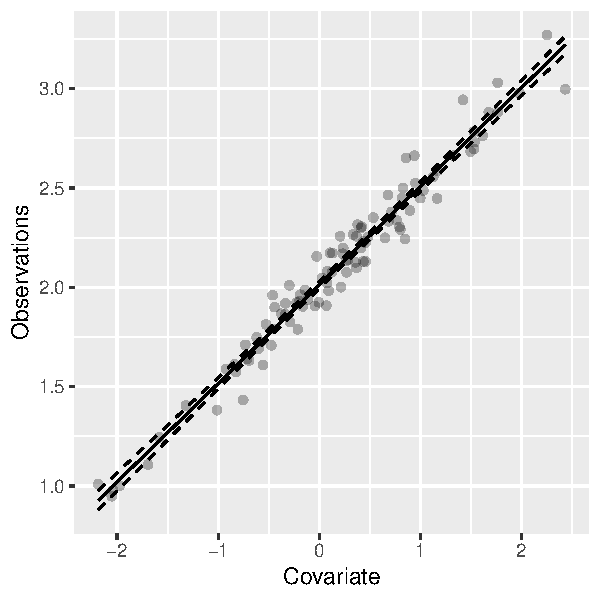
\includegraphics{day1_practical_files/figure-pdf/unnamed-chunk-11-1.pdf}

}

\caption{Data and 95\% credible intervals}

\end{figure}%

\subsection{R Code}

\begin{Shaded}
\begin{Highlighting}[]
\NormalTok{pred }\SpecialCharTok{\%\textgreater{}\%} \FunctionTok{ggplot}\NormalTok{() }\SpecialCharTok{+} 
  \FunctionTok{geom\_point}\NormalTok{(}\FunctionTok{aes}\NormalTok{(x,y), }\AttributeTok{alpha =} \FloatTok{0.3}\NormalTok{) }\SpecialCharTok{+}
  \FunctionTok{geom\_line}\NormalTok{(}\FunctionTok{aes}\NormalTok{(x,mean)) }\SpecialCharTok{+}
  \FunctionTok{geom\_line}\NormalTok{(}\FunctionTok{aes}\NormalTok{(x, q0}\FloatTok{.025}\NormalTok{), }\AttributeTok{linetype =} \StringTok{"dashed"}\NormalTok{)}\SpecialCharTok{+}
  \FunctionTok{geom\_line}\NormalTok{(}\FunctionTok{aes}\NormalTok{(x, q0}\FloatTok{.975}\NormalTok{), }\AttributeTok{linetype =} \StringTok{"dashed"}\NormalTok{)}\SpecialCharTok{+}
  \FunctionTok{xlab}\NormalTok{(}\StringTok{"Covariate"}\NormalTok{) }\SpecialCharTok{+} \FunctionTok{ylab}\NormalTok{(}\StringTok{"Observations"}\NormalTok{)}
\end{Highlighting}
\end{Shaded}

\begin{tcolorbox}[enhanced jigsaw, toprule=.15mm, coltitle=black, opacitybacktitle=0.6, colframe=quarto-callout-warning-color-frame, breakable, colback=white, opacityback=0, leftrule=.75mm, arc=.35mm, rightrule=.15mm, bottomrule=.15mm, colbacktitle=quarto-callout-warning-color!10!white, title={Task}, toptitle=1mm, titlerule=0mm, left=2mm, bottomtitle=1mm]

Generate predictions for a new observation with \(x_0 = 0.45\)

Take hint

You can create a new data frame containing the new observation \(x_0\)
and then use the \texttt{predict} function.

Click here to see the solution

\begin{Shaded}
\begin{Highlighting}[]
\NormalTok{new\_data }\OtherTok{=} \FunctionTok{data.frame}\NormalTok{(}\AttributeTok{x =} \FloatTok{0.45}\NormalTok{)}
\NormalTok{pred }\OtherTok{=} \FunctionTok{predict}\NormalTok{(fit.lm, new\_data, }\SpecialCharTok{\textasciitilde{}}\NormalTok{ beta\_0 }\SpecialCharTok{+}\NormalTok{ beta\_1,}
               \AttributeTok{n.samples =} \DecValTok{1000}\NormalTok{)}
\end{Highlighting}
\end{Shaded}

\end{tcolorbox}

\subsection{Linear Mixed Model}\label{linear-mixed-model}

In this practical we will:

\begin{itemize}
\tightlist
\item
  Understand the basic structure of a Linear Mixed Model (LLM)
\item
  Simulate data from a LMM
\item
  Learn how to fit a LMM with \texttt{inlabru} and predict from the
  model.
\end{itemize}

Consider the a simple linear regression model except with the addition
that the data that comes in groups. Suppose that we want to include a
random effect for each group \(j\) (equivalent to adding a group random
intercept). The model is then: \[
 y_{ij}  = \beta_0 + \beta_1 x_i + u_j + \epsilon_{ij} ~~~  \text{for}~i = 1,\ldots,N~ \text{and}~ j = 1,\ldots,m.
\]

Here the random group effect is given by the variable
\(u_j \sim \mathcal{N}(0, \tau^{-1}_u)\) with \(\tau_u = 1/\sigma^2_u\)
describing the variability between groups (i.e., how much the group
means differ from the overall mean). Then,
\(\epsilon_j \sim \mathcal{N}(0, \tau^{-1}_\epsilon)\) denotes the
residuals of the model and \(\tau_\epsilon = 1/\sigma^2_\epsilon\)
captures how much individual observations deviate from their group mean
(i.e., variability within group).

The model design matrix for the random effect has one row for each
observation (this is equivalent to a random intercept model). The row of
the design matrix associated with the \(ij\)-th observation consists of
zeros except for the element associated with \(u_j\), which has a one.

\[
\pmb{\eta} = \pmb{A}\pmb{u} = \pmb{A}_1\pmb{u}_1 + \pmb{A}_2\pmb{u}_2 + \pmb{A}_3\pmb{u}_3
\]

\begin{tcolorbox}[enhanced jigsaw, toprule=.15mm, coltitle=black, opacitybacktitle=0.6, colframe=quarto-callout-note-color-frame, breakable, colback=white, opacityback=0, leftrule=.75mm, arc=.35mm, rightrule=.15mm, bottomrule=.15mm, colbacktitle=quarto-callout-note-color!10!white, title={Supplementary material: LMM as a LGM}, toptitle=1mm, titlerule=0mm, left=2mm, bottomtitle=1mm]

In matrix form, the linear mixed model for the \emph{j}-th group can be
written as:

\[ \overbrace{\mathbf{y}_j}^{ N \times 1} = \overbrace{X_j}^{ N \times 2} \underbrace{\beta}_{1\times 1} + \overbrace{Z_j}^{n_j \times 1} \underbrace{u_j}_{1\times1} + \overbrace{\epsilon_j}^{n_j \times 1}, \]

In a latent Gaussian model (LGM) formulation the mixed model predictor
for the \emph{i}-th observation can be written as :

\[
\eta_i = \beta_0 + \beta_1 x_i + \sum_k^K f_k(u_j)
\]

where \(f_k(u_j) = u_j\) since there's only one random effect per group
(i.e., a random intercept for group \(j\)). The fixed effects
\((\beta_0,\beta_1)\) are assigned Gaussian priors (e.g.,
\(\beta \sim \mathcal{N}(0,\tau_\beta^{-1})\)). The random effects
\(\mathbf{u} = (u_1,\ldots,u_m)^T\) follow a Gaussian density
\(\mathcal{N}(0,\mathbf{Q}_u^{-1})\) where
\(\mathbf{Q}_u = \tau_u\mathbf{I}_m\) is the precision matrix for the
random intercepts. Then, the components for the LGM are the following:

\begin{itemize}
\item
  Latent field given by

  \[
  \begin{bmatrix} \beta \\\mathbf{u} 
  \end{bmatrix} \sim \mathcal{N}\left(\mathbf{0},\begin{bmatrix}\tau_\beta^{-1}\mathbf{I}_2&\mathbf{0}\\\mathbf{0} &\tau_u^{-1}\mathbf{I}_m\end{bmatrix}\right)
  \]
\item
  Likelihood:

  \[
  y_i \sim \mathcal{N}(\eta_i,\tau_{\epsilon}^{-1})
  \]
\item
  Hyperparameters:

  \begin{itemize}
  \tightlist
  \item
    \(\tau_u\sim\mathrm{Gamma}(a,b)\)
  \item
    \(\tau_\epsilon \sim \mathrm{Gamma}(c,d)\)
  \end{itemize}
\end{itemize}

\end{tcolorbox}

\subsubsection{\texorpdfstring{\textbf{Simulate example
data}}{Simulate example data}}\label{simulate-example-data-1}

\begin{Shaded}
\begin{Highlighting}[]
\FunctionTok{set.seed}\NormalTok{(}\DecValTok{12}\NormalTok{)}
\NormalTok{beta }\OtherTok{=} \FunctionTok{c}\NormalTok{(}\FloatTok{1.5}\NormalTok{,}\DecValTok{1}\NormalTok{)}
\NormalTok{sd\_error }\OtherTok{=} \DecValTok{1}
\NormalTok{tau\_group }\OtherTok{=} \DecValTok{1}

\NormalTok{n }\OtherTok{=} \DecValTok{100}
\NormalTok{n.groups }\OtherTok{=} \DecValTok{5}
\NormalTok{x }\OtherTok{=} \FunctionTok{rnorm}\NormalTok{(n)}
\NormalTok{v }\OtherTok{=} \FunctionTok{rnorm}\NormalTok{(n.groups, }\AttributeTok{sd =}\NormalTok{ tau\_group}\SpecialCharTok{\^{}}\NormalTok{\{}\SpecialCharTok{{-}}\DecValTok{1}\SpecialCharTok{/}\DecValTok{2}\NormalTok{\})}
\NormalTok{y }\OtherTok{=}\NormalTok{ beta[}\DecValTok{1}\NormalTok{] }\SpecialCharTok{+}\NormalTok{ beta[}\DecValTok{2}\NormalTok{] }\SpecialCharTok{*}\NormalTok{ x }\SpecialCharTok{+} \FunctionTok{rnorm}\NormalTok{(n, }\AttributeTok{sd =}\NormalTok{ sd\_error) }\SpecialCharTok{+}
  \FunctionTok{rep}\NormalTok{(v, }\AttributeTok{each =} \DecValTok{20}\NormalTok{)}

\NormalTok{df }\OtherTok{=} \FunctionTok{data.frame}\NormalTok{(}\AttributeTok{y =}\NormalTok{ y, }\AttributeTok{x =}\NormalTok{ x, }\AttributeTok{j =} \FunctionTok{rep}\NormalTok{(}\DecValTok{1}\SpecialCharTok{:}\DecValTok{5}\NormalTok{, }\AttributeTok{each =} \DecValTok{20}\NormalTok{))  }
\end{Highlighting}
\end{Shaded}

Note that \texttt{inlabru} expects an integer indexing variable to label
the groups.

\begin{Shaded}
\begin{Highlighting}[]
\FunctionTok{ggplot}\NormalTok{(df) }\SpecialCharTok{+}
  \FunctionTok{geom\_point}\NormalTok{(}\FunctionTok{aes}\NormalTok{(}\AttributeTok{x =}\NormalTok{ x, }\AttributeTok{colour =} \FunctionTok{factor}\NormalTok{(j), }\AttributeTok{y =}\NormalTok{ y)) }\SpecialCharTok{+}
  \FunctionTok{theme\_classic}\NormalTok{() }\SpecialCharTok{+}
  \FunctionTok{scale\_colour\_discrete}\NormalTok{(}\StringTok{"Group"}\NormalTok{)}
\end{Highlighting}
\end{Shaded}

\begin{figure}[H]

{\centering 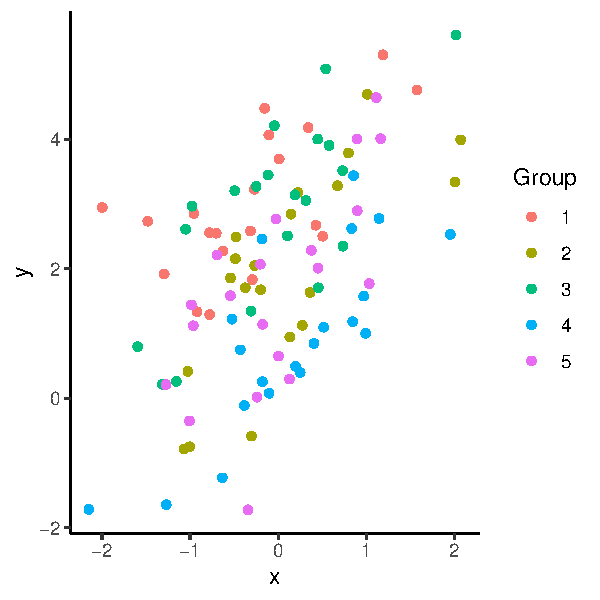
\includegraphics{day1_practical_files/figure-pdf/plot_data_lmm-1.pdf}

}

\caption{Data for the linear mixed model example with 5 groups}

\end{figure}%

\subsubsection{\texorpdfstring{Fitting a LMM in
\texttt{inlabru}}{Fitting a LMM in inlabru}}\label{fitting-a-lmm-in-inlabru}

\begin{center}\rule{0.5\linewidth}{0.5pt}\end{center}

\textbf{Defining model components and observational model}

In order to specify this model we must use the \texttt{group} argument
to tell \texttt{inlabru} which variable indexes the groups. The
\texttt{model\ =\ "iid"} tells INLA that the groups are independent from
one another.

\begin{Shaded}
\begin{Highlighting}[]
\CommentTok{\# Define model components}
\NormalTok{cmp }\OtherTok{=}  \ErrorTok{\textasciitilde{}} \SpecialCharTok{{-}}\DecValTok{1} \SpecialCharTok{+} \FunctionTok{beta\_0}\NormalTok{(}\DecValTok{1}\NormalTok{) }\SpecialCharTok{+} \FunctionTok{beta\_1}\NormalTok{(x, }\AttributeTok{model =} \StringTok{"linear"}\NormalTok{) }\SpecialCharTok{+}
  \FunctionTok{u}\NormalTok{(j, }\AttributeTok{model =} \StringTok{"iid"}\NormalTok{)}
\end{Highlighting}
\end{Shaded}

The group variable is indexed by column \texttt{j} in the dataset. We
have chosen to name this component \texttt{v()} to connect with the
mathematical notation that we used above.

\begin{Shaded}
\begin{Highlighting}[]
\CommentTok{\# Construct likelihood}
\NormalTok{lik }\OtherTok{=}  \FunctionTok{like}\NormalTok{(}\AttributeTok{formula =}\NormalTok{ y }\SpecialCharTok{\textasciitilde{}}\NormalTok{.,}
            \AttributeTok{family =} \StringTok{"gaussian"}\NormalTok{,}
            \AttributeTok{data =}\NormalTok{ df)}
\end{Highlighting}
\end{Shaded}

\textbf{Fitting the model}

The model can be fitted exactly as in the previous examples by using the
\texttt{bru} function with the components and likelihood objects.

\begin{Shaded}
\begin{Highlighting}[]
\NormalTok{fit }\OtherTok{=} \FunctionTok{bru}\NormalTok{(cmp, lik)}
\FunctionTok{summary}\NormalTok{(fit)}
\DocumentationTok{\#\# inlabru version: 2.12.0}
\DocumentationTok{\#\# INLA version: 25.06.22{-}1}
\DocumentationTok{\#\# Components:}
\DocumentationTok{\#\# beta\_0: main = linear(1), group = exchangeable(1L), replicate = iid(1L), NULL}
\DocumentationTok{\#\# beta\_1: main = linear(x), group = exchangeable(1L), replicate = iid(1L), NULL}
\DocumentationTok{\#\# u: main = iid(j), group = exchangeable(1L), replicate = iid(1L), NULL}
\DocumentationTok{\#\# Likelihoods:}
\DocumentationTok{\#\#   Family: \textquotesingle{}gaussian\textquotesingle{}}
\DocumentationTok{\#\#     Tag: \textquotesingle{}\textquotesingle{}}
\DocumentationTok{\#\#     Data class: \textquotesingle{}data.frame\textquotesingle{}}
\DocumentationTok{\#\#     Response class: \textquotesingle{}numeric\textquotesingle{}}
\DocumentationTok{\#\#     Predictor: y \textasciitilde{} .}
\DocumentationTok{\#\#     Used components: effects[beta\_0, beta\_1, u], latent[]}
\DocumentationTok{\#\# Time used:}
\DocumentationTok{\#\#     Pre = 0.357, Running = 0.289, Post = 0.177, Total = 0.823 }
\DocumentationTok{\#\# Fixed effects:}
\DocumentationTok{\#\#         mean    sd 0.025quant 0.5quant 0.975quant  mode    kld}
\DocumentationTok{\#\# beta\_0 2.108 0.438      1.229    2.108      2.986 2.108  7.745}
\DocumentationTok{\#\# beta\_1 1.172 0.120      0.936    1.172      1.407 1.172 41.046}
\DocumentationTok{\#\# }
\DocumentationTok{\#\# Random effects:}
\DocumentationTok{\#\#   Name     Model}
\DocumentationTok{\#\#     u IID model}
\DocumentationTok{\#\# }
\DocumentationTok{\#\# Model hyperparameters:}
\DocumentationTok{\#\#                                          mean    sd 0.025quant 0.5quant}
\DocumentationTok{\#\# Precision for the Gaussian observations 0.995 0.144      0.738    0.986}
\DocumentationTok{\#\# Precision for u                         1.613 1.060      0.369    1.356}
\DocumentationTok{\#\#                                         0.975quant  mode}
\DocumentationTok{\#\# Precision for the Gaussian observations       1.30 0.971}
\DocumentationTok{\#\# Precision for u                               4.35 0.918}
\DocumentationTok{\#\# }
\DocumentationTok{\#\# Deviance Information Criterion (DIC) ...............: 294.30}
\DocumentationTok{\#\# Deviance Information Criterion (DIC, saturated) ....: 109.03}
\DocumentationTok{\#\# Effective number of parameters .....................: 6.72}
\DocumentationTok{\#\# }
\DocumentationTok{\#\# Watanabe{-}Akaike information criterion (WAIC) ...: 294.32}
\DocumentationTok{\#\# Effective number of parameters .................: 6.34}
\DocumentationTok{\#\# }
\DocumentationTok{\#\# Marginal log{-}Likelihood:  {-}179.93 }
\DocumentationTok{\#\#  is computed }
\DocumentationTok{\#\# Posterior summaries for the linear predictor and the fitted values are computed}
\DocumentationTok{\#\# (Posterior marginals needs also \textquotesingle{}control.compute=list(return.marginals.predictor=TRUE)\textquotesingle{})}
\end{Highlighting}
\end{Shaded}

\subsubsection{Model predictions}\label{model-predictions}

To compute model predictions we can create a \texttt{data.frame}
containing a range of values of covariate where we want the response to
be predicted for each group. Then we simply call the predict function
while spe

\begin{Shaded}
\begin{Highlighting}[]
\CommentTok{\# New data}
\NormalTok{xpred }\OtherTok{=} \FunctionTok{seq}\NormalTok{(}\FunctionTok{range}\NormalTok{(x)[}\DecValTok{1}\NormalTok{], }\FunctionTok{range}\NormalTok{(x)[}\DecValTok{2}\NormalTok{], }\AttributeTok{length.out =} \DecValTok{100}\NormalTok{)}
\NormalTok{j }\OtherTok{=} \DecValTok{1}\SpecialCharTok{:}\NormalTok{n.groups}
\NormalTok{pred\_data }\OtherTok{=} \FunctionTok{expand.grid}\NormalTok{(}\AttributeTok{x =}\NormalTok{ xpred, }\AttributeTok{j =}\NormalTok{ j)}
\NormalTok{pred }\OtherTok{=} \FunctionTok{predict}\NormalTok{(fit, pred\_data, }\AttributeTok{formula =} \SpecialCharTok{\textasciitilde{}}\NormalTok{ beta\_0 }\SpecialCharTok{+}\NormalTok{ beta\_1 }\SpecialCharTok{+}\NormalTok{ u) }


\NormalTok{pred }\SpecialCharTok{\%\textgreater{}\%}
  \FunctionTok{ggplot}\NormalTok{(}\FunctionTok{aes}\NormalTok{(}\AttributeTok{x=}\NormalTok{x,}\AttributeTok{y=}\NormalTok{mean,}\AttributeTok{color=}\FunctionTok{factor}\NormalTok{(j)))}\SpecialCharTok{+}
  \FunctionTok{geom\_line}\NormalTok{()}\SpecialCharTok{+}
  \FunctionTok{geom\_ribbon}\NormalTok{(}\FunctionTok{aes}\NormalTok{(x,}\AttributeTok{ymin =}\NormalTok{ q0}\FloatTok{.025}\NormalTok{, }\AttributeTok{ymax=}\NormalTok{ q0}\FloatTok{.975}\NormalTok{,}\AttributeTok{fill=}\FunctionTok{factor}\NormalTok{(j)), }\AttributeTok{alpha =} \FloatTok{0.5}\NormalTok{) }\SpecialCharTok{+} 
  \FunctionTok{geom\_point}\NormalTok{(}\AttributeTok{data=}\NormalTok{df,}\FunctionTok{aes}\NormalTok{(}\AttributeTok{x=}\NormalTok{x,}\AttributeTok{y=}\NormalTok{y,}\AttributeTok{colour=}\FunctionTok{factor}\NormalTok{(j)))}\SpecialCharTok{+}
  \FunctionTok{facet\_wrap}\NormalTok{(}\SpecialCharTok{\textasciitilde{}}\NormalTok{j)}
\end{Highlighting}
\end{Shaded}

\begin{center}
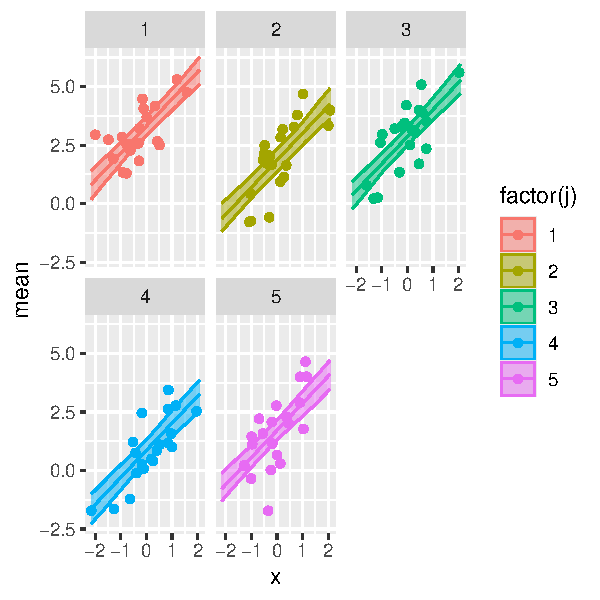
\includegraphics{day1_practical_files/figure-pdf/unnamed-chunk-31-1.pdf}
\end{center}

\begin{tcolorbox}[enhanced jigsaw, toprule=.15mm, coltitle=black, opacitybacktitle=0.6, colframe=quarto-callout-tip-color-frame, breakable, colback=white, opacityback=0, leftrule=.75mm, arc=.35mm, rightrule=.15mm, bottomrule=.15mm, colbacktitle=quarto-callout-tip-color!10!white, title={Question}, toptitle=1mm, titlerule=0mm, left=2mm, bottomtitle=1mm]

Suppose that we are also interested in including random slopes into our
model. Assuming intercept and slopes are independent, can your write
down the linear predictor and the components of this model as a LGM?

Give me a hint

In general, the mixed model predictor can decomposed as:

\[ \pmb{\eta} = X\beta + Z\mathbf{u} \]

Where \(X\) is a \(n \times p\) design matrix and \(\beta\) the
corresponding \emph{p}-dimensional vector of fixed effects. Then \(Z\)
is a \(n\times q_J\) design matrix for the \(q_J\) random effects and
\(J\) groups; \(\mathbf{v}\) is then a \(q_J \times 1\) vector of \(q\)
random effects for the \(J\) groups. In a latent Gaussian model (LGM)
formulation this can be written as:

\[ \eta_i = \beta_0 + \sum\beta_j x_{ij} + \sum_k f(k) (u_{ij}) \]

See Solution

\begin{itemize}
\item
  The linear predictor is given by

  \[
  \eta_i = \beta_0 + \beta_1x_i + u_{0j} + u_{1j}x_i
  \]
\item
  Latent field defined by:

  \begin{itemize}
  \item
    \(\beta \sim \mathcal{N}(0,\tau_\beta^{-1})\)
  \item
    \(\mathbf{u}_j = \begin{bmatrix}u_{0j} \\ u_{1j}\end{bmatrix}, \mathbf{u}_j \sim \mathcal{N}(\mathbf{0},\mathbf{Q}_u^{-1})\)
    where the precision matrix is a block-diagonal matrix with entries
    \(\mathbf{Q}_u= \begin{bmatrix}\tau_{u_0} & {0} \\{0} & \tau_{u_1}\end{bmatrix}\)
  \end{itemize}
\item
  The hyperparameters are then:

  \begin{itemize}
  \tightlist
  \item
    \(\tau_{u_0},\tau_{u_1} \text{and}~\tau_\epsilon\)
  \end{itemize}
\end{itemize}

To fit this model in \texttt{inlabru} we can simply modify the model
components as follows:

\begin{Shaded}
\begin{Highlighting}[]
\NormalTok{cmp }\OtherTok{=}  \ErrorTok{\textasciitilde{}} \SpecialCharTok{{-}}\DecValTok{1} \SpecialCharTok{+} \FunctionTok{beta\_0}\NormalTok{(}\DecValTok{1}\NormalTok{) }\SpecialCharTok{+} \FunctionTok{beta\_1}\NormalTok{(x, }\AttributeTok{model =} \StringTok{"linear"}\NormalTok{) }\SpecialCharTok{+}
  \FunctionTok{u0}\NormalTok{(j, }\AttributeTok{model =} \StringTok{"iid"}\NormalTok{) }\SpecialCharTok{+} \FunctionTok{u1}\NormalTok{(j,x, }\AttributeTok{model =} \StringTok{"iid"}\NormalTok{)}
\end{Highlighting}
\end{Shaded}

\end{tcolorbox}

\subsection{Generalized Linear Model}\label{sec-genlinmodel}

In this practical we will:

\begin{itemize}
\tightlist
\item
  Simulate non-Gaussian data
\item
  Learn how to fit a generalised linear model with \texttt{inlabru}
\item
  Generate predictions from the model
\end{itemize}

A generalised linear model allows for the data likelihood to be
non-Gaussian. In this example we have a discrete response variable which
we model using a Poisson distribution. Thus, we assume that our data \[
y_i \sim \text{Poisson}(\lambda_i)
\] with rate parameter \(\lambda_i\) which, using a log link, has
associated predictor \[
\eta_i = \log \lambda_i = \beta_0 + \beta_1 x_i 
\] with parameters \(\beta_0\) and \(\beta_1\), and covariate \(x\).
This is identical in form to the predictor in
Section~\ref{sec-linmodel}. The only difference is now we must specify a
different data likelihood.

\subsubsection{\texorpdfstring{\textbf{Simulate example
data}}{Simulate example data}}\label{simulate-example-data-2}

This code generates 100 samples of covariate \texttt{x} and data
\texttt{y}.

\begin{Shaded}
\begin{Highlighting}[]
\FunctionTok{set.seed}\NormalTok{(}\DecValTok{123}\NormalTok{)}
\NormalTok{n }\OtherTok{=} \DecValTok{100}
\NormalTok{beta }\OtherTok{=} \FunctionTok{c}\NormalTok{(}\DecValTok{1}\NormalTok{,}\DecValTok{1}\NormalTok{)}
\NormalTok{x }\OtherTok{=} \FunctionTok{rnorm}\NormalTok{(n)}
\NormalTok{lambda }\OtherTok{=} \FunctionTok{exp}\NormalTok{(beta[}\DecValTok{1}\NormalTok{] }\SpecialCharTok{+}\NormalTok{ beta[}\DecValTok{2}\NormalTok{] }\SpecialCharTok{*}\NormalTok{ x)}
\NormalTok{y }\OtherTok{=} \FunctionTok{rpois}\NormalTok{(n, }\AttributeTok{lambda  =}\NormalTok{ lambda)}
\NormalTok{df }\OtherTok{=} \FunctionTok{data.frame}\NormalTok{(}\AttributeTok{y =}\NormalTok{ y, }\AttributeTok{x =}\NormalTok{ x)  }
\end{Highlighting}
\end{Shaded}

\subsubsection{\texorpdfstring{Fitting a GLM in
\texttt{inlabru}}{Fitting a GLM in inlabru}}\label{fitting-a-glm-in-inlabru}

\begin{center}\rule{0.5\linewidth}{0.5pt}\end{center}

\textbf{Define model components and likelihood}

Since the predictor is the same as Section~\ref{sec-linmodel}, we can
use the same component definition:

\begin{Shaded}
\begin{Highlighting}[]
\NormalTok{cmp }\OtherTok{=}  \ErrorTok{\textasciitilde{}} \SpecialCharTok{{-}}\DecValTok{1} \SpecialCharTok{+} \FunctionTok{beta\_0}\NormalTok{(}\DecValTok{1}\NormalTok{) }\SpecialCharTok{+} \FunctionTok{beta\_1}\NormalTok{(x, }\AttributeTok{model =} \StringTok{"linear"}\NormalTok{)}
\end{Highlighting}
\end{Shaded}

However, when building the observation model likelihood we must now
specify the Poisson likelihood using the \texttt{family} argument (the
default link function for this family is the \(\log\) link).

\begin{Shaded}
\begin{Highlighting}[]
\NormalTok{lik }\OtherTok{=}  \FunctionTok{bru\_obs}\NormalTok{(}\AttributeTok{formula =}\NormalTok{ y }\SpecialCharTok{\textasciitilde{}}\NormalTok{.,}
            \AttributeTok{family =} \StringTok{"poisson"}\NormalTok{,}
            \AttributeTok{data =}\NormalTok{ df)}
\end{Highlighting}
\end{Shaded}

\textbf{Fit the model}

Once the likelihood object is constructed, fitting the model is exactly
the same process as in Section~\ref{sec-linmodel}.

\begin{Shaded}
\begin{Highlighting}[]
\NormalTok{fit\_glm }\OtherTok{=} \FunctionTok{bru}\NormalTok{(cmp, lik)}
\end{Highlighting}
\end{Shaded}

And model summaries can be viewed using

\begin{Shaded}
\begin{Highlighting}[]
\FunctionTok{summary}\NormalTok{(fit\_glm)}
\end{Highlighting}
\end{Shaded}

\begin{verbatim}
inlabru version: 2.12.0
INLA version: 25.06.22-1
Components:
beta_0: main = linear(1), group = exchangeable(1L), replicate = iid(1L), NULL
beta_1: main = linear(x), group = exchangeable(1L), replicate = iid(1L), NULL
Likelihoods:
  Family: 'poisson'
    Tag: ''
    Data class: 'data.frame'
    Response class: 'integer'
    Predictor: y ~ .
    Used components: effects[beta_0, beta_1], latent[]
Time used:
    Pre = 0.276, Running = 0.218, Post = 0.0483, Total = 0.542 
Fixed effects:
        mean    sd 0.025quant 0.5quant 0.975quant  mode     kld
beta_0 0.915 0.071      0.775    0.915      1.054 0.915  90.413
beta_1 1.048 0.056      0.938    1.048      1.157 1.048 167.611

Deviance Information Criterion (DIC) ...............: 386.39
Deviance Information Criterion (DIC, saturated) ....: 120.67
Effective number of parameters .....................: 2.00

Watanabe-Akaike information criterion (WAIC) ...: 387.33
Effective number of parameters .................: 2.73

Marginal log-Likelihood:  -204.02 
 is computed 
Posterior summaries for the linear predictor and the fitted values are computed
(Posterior marginals needs also 'control.compute=list(return.marginals.predictor=TRUE)')
\end{verbatim}

\subsubsection{Generate model
predictions}\label{generate-model-predictions-1}

\begin{center}\rule{0.5\linewidth}{0.5pt}\end{center}

To generate new predictions we must provide a data frame that contains
the covariate values for \(x\) at which we want to predict.

This code block generates predictions for the data we used to fit the
model (contained in \texttt{df\$x}) as well as 10 new covariate values
sampled from a uniform distribution \texttt{runif(10)}.

\begin{Shaded}
\begin{Highlighting}[]
\CommentTok{\# Define new data, set to NA the values for prediction}

\NormalTok{new\_data }\OtherTok{=} \FunctionTok{data.frame}\NormalTok{(}\AttributeTok{x =} \FunctionTok{c}\NormalTok{(df}\SpecialCharTok{$}\NormalTok{x, }\FunctionTok{runif}\NormalTok{(}\DecValTok{10}\NormalTok{)),}
                      \AttributeTok{y =} \FunctionTok{c}\NormalTok{(df}\SpecialCharTok{$}\NormalTok{y, }\FunctionTok{rep}\NormalTok{(}\ConstantTok{NA}\NormalTok{,}\DecValTok{10}\NormalTok{)))}

\CommentTok{\# Define predictor formula}
\NormalTok{pred\_fml }\OtherTok{\textless{}{-}} \ErrorTok{\textasciitilde{}} \FunctionTok{exp}\NormalTok{(beta\_0 }\SpecialCharTok{+}\NormalTok{ beta\_1)}

\CommentTok{\# Generate predictions}
\NormalTok{pred\_glm }\OtherTok{\textless{}{-}} \FunctionTok{predict}\NormalTok{(fit\_glm, new\_data, pred\_fml)}
\end{Highlighting}
\end{Shaded}

Since we used a log link (which is the default for
\texttt{family\ =\ "poisson"}), we want to predict the exponential of
the predictor. We specify this using a general \texttt{R} expression
using the formula syntax.

\begin{tcolorbox}[enhanced jigsaw, toprule=.15mm, coltitle=black, opacitybacktitle=0.6, colframe=quarto-callout-note-color-frame, breakable, colback=white, opacityback=0, leftrule=.75mm, arc=.35mm, rightrule=.15mm, bottomrule=.15mm, colbacktitle=quarto-callout-note-color!10!white, title=\textcolor{quarto-callout-note-color}{\faInfo}\hspace{0.5em}{Note}, toptitle=1mm, titlerule=0mm, left=2mm, bottomtitle=1mm]

Note that the \texttt{predict} function will call the component names
(i.e.~the ``labels'') that were decided when defining the model.

\end{tcolorbox}

Since the component definition is looking for a covariate named \(x\),
all we need to provide is a data frame that contains one, and the
software does the rest.

\subsection{Plot}

\begin{figure}[H]

{\centering 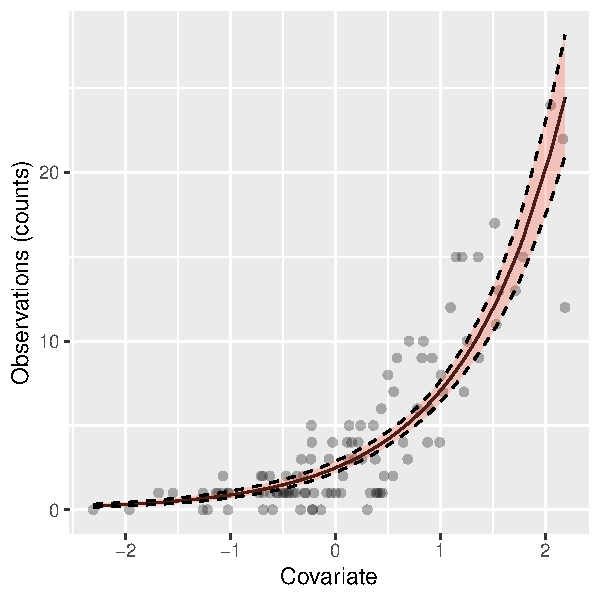
\includegraphics{day1_practical_files/figure-pdf/unnamed-chunk-49-1.pdf}

}

\caption{Data and 95\% credible intervals}

\end{figure}%

\subsection{R Code}

\begin{Shaded}
\begin{Highlighting}[]
\NormalTok{pred\_glm }\SpecialCharTok{\%\textgreater{}\%} \FunctionTok{ggplot}\NormalTok{() }\SpecialCharTok{+} 
  \FunctionTok{geom\_point}\NormalTok{(}\FunctionTok{aes}\NormalTok{(x,y), }\AttributeTok{alpha =} \FloatTok{0.3}\NormalTok{) }\SpecialCharTok{+}
  \FunctionTok{geom\_line}\NormalTok{(}\FunctionTok{aes}\NormalTok{(x,mean)) }\SpecialCharTok{+}
    \FunctionTok{geom\_ribbon}\NormalTok{(}\FunctionTok{aes}\NormalTok{(}\AttributeTok{x =}\NormalTok{ x, }\AttributeTok{ymax =}\NormalTok{ q0}\FloatTok{.975}\NormalTok{, }\AttributeTok{ymin =}\NormalTok{ q0}\FloatTok{.025}\NormalTok{),}\AttributeTok{fill =} \StringTok{"tomato"}\NormalTok{, }\AttributeTok{alpha =} \FloatTok{0.3}\NormalTok{)}\SpecialCharTok{+}
  \FunctionTok{xlab}\NormalTok{(}\StringTok{"Covariate"}\NormalTok{) }\SpecialCharTok{+} \FunctionTok{ylab}\NormalTok{(}\StringTok{"Observations (counts)"}\NormalTok{)}
\end{Highlighting}
\end{Shaded}

\begin{tcolorbox}[enhanced jigsaw, toprule=.15mm, coltitle=black, opacitybacktitle=0.6, colframe=quarto-callout-warning-color-frame, breakable, colback=white, opacityback=0, leftrule=.75mm, arc=.35mm, rightrule=.15mm, bottomrule=.15mm, colbacktitle=quarto-callout-warning-color!10!white, title={Task}, toptitle=1mm, titlerule=0mm, left=2mm, bottomtitle=1mm]

Suppose a binary response such that

\[
    \begin{aligned}
y_i &\sim \mathrm{Bernoulli}(\psi_i)\\
\eta_i &= \mathrm{logit}(\psi_i) = \alpha_0 +\alpha_1 \times w_i 
\end{aligned}
\] Using the following simulated data, use \texttt{inlabru} to fit the
logistic regression above. Then, plot the predictions for the data used
to fit the model along with 10 new covariate values

\begin{Shaded}
\begin{Highlighting}[]
\FunctionTok{set.seed}\NormalTok{(}\DecValTok{123}\NormalTok{)}
\NormalTok{n }\OtherTok{=} \DecValTok{100}
\NormalTok{alpha }\OtherTok{=} \FunctionTok{c}\NormalTok{(}\FloatTok{0.5}\NormalTok{,}\FloatTok{1.5}\NormalTok{)}
\NormalTok{w }\OtherTok{=} \FunctionTok{rnorm}\NormalTok{(n)}
\NormalTok{psi }\OtherTok{=} \FunctionTok{plogis}\NormalTok{(alpha[}\DecValTok{1}\NormalTok{] }\SpecialCharTok{+}\NormalTok{ alpha[}\DecValTok{2}\NormalTok{] }\SpecialCharTok{*}\NormalTok{ w)}
\NormalTok{y }\OtherTok{=} \FunctionTok{rbinom}\NormalTok{(}\AttributeTok{n =}\NormalTok{ n, }\AttributeTok{size =} \DecValTok{1}\NormalTok{, }\AttributeTok{prob =}\NormalTok{  psi) }\CommentTok{\# set size = 1 to draw binary observations}
\NormalTok{df\_logis }\OtherTok{=} \FunctionTok{data.frame}\NormalTok{(}\AttributeTok{y =}\NormalTok{ y, }\AttributeTok{w =}\NormalTok{ w)  }
\end{Highlighting}
\end{Shaded}

Here we use the logit link function
\(\mathrm{logit}(x) = \log\left(\frac{x}{1-x}\right)\)
(\texttt{plogis()} function in R) to link the linear predictor to the
probabilities \(\psi\).

Take hint

You can set \texttt{family\ =\ "binomial"} for binary responses and the
\texttt{plogis()} function for computing the predicted values.

\begin{tcolorbox}[enhanced jigsaw, toprule=.15mm, coltitle=black, opacitybacktitle=0.6, colframe=quarto-callout-note-color-frame, breakable, colback=white, opacityback=0, leftrule=.75mm, arc=.35mm, rightrule=.15mm, bottomrule=.15mm, colbacktitle=quarto-callout-note-color!10!white, title=\textcolor{quarto-callout-note-color}{\faInfo}\hspace{0.5em}{Note}, toptitle=1mm, titlerule=0mm, left=2mm, bottomtitle=1mm]

The Bernoulli distribution is equivalent to a
\(\mathrm{Binomial}(1, \psi)\) pmf. If you have proportional data
(e.g.~no. successes/no. trials) you can specify the number of events as
your response and then the number of trials via the
\texttt{Ntrials\ =\ n} argument of the \texttt{bru\_obs} function (where
\texttt{n} is the known vector of trials in your data set).

\end{tcolorbox}

Click here to see the solution

\begin{Shaded}
\begin{Highlighting}[]
\CommentTok{\# Model components}
\NormalTok{cmp\_logis }\OtherTok{=}  \ErrorTok{\textasciitilde{}} \SpecialCharTok{{-}}\DecValTok{1} \SpecialCharTok{+} \FunctionTok{alpha\_0}\NormalTok{(}\DecValTok{1}\NormalTok{) }\SpecialCharTok{+} \FunctionTok{alpha\_1}\NormalTok{(w, }\AttributeTok{model =} \StringTok{"linear"}\NormalTok{)}
\CommentTok{\# Model likelihood}
\NormalTok{lik\_logis }\OtherTok{=}  \FunctionTok{bru\_obs}\NormalTok{(}\AttributeTok{formula =}\NormalTok{ y }\SpecialCharTok{\textasciitilde{}}\NormalTok{.,}
            \AttributeTok{family =} \StringTok{"binomial"}\NormalTok{,}
            \AttributeTok{data =}\NormalTok{ df\_logis)}
\CommentTok{\# fit the model}
\NormalTok{fit\_logis }\OtherTok{\textless{}{-}} \FunctionTok{bru}\NormalTok{(cmp\_logis,lik\_logis)}

\CommentTok{\# Define data for prediction}
\NormalTok{new\_data }\OtherTok{=} \FunctionTok{data.frame}\NormalTok{(}\AttributeTok{w =} \FunctionTok{c}\NormalTok{(df\_logis}\SpecialCharTok{$}\NormalTok{w, }\FunctionTok{runif}\NormalTok{(}\DecValTok{10}\NormalTok{)),}
                      \AttributeTok{y =} \FunctionTok{c}\NormalTok{(df\_logis}\SpecialCharTok{$}\NormalTok{y, }\FunctionTok{rep}\NormalTok{(}\ConstantTok{NA}\NormalTok{,}\DecValTok{10}\NormalTok{)))}
\CommentTok{\# Define predictor formula}
\NormalTok{pred\_fml }\OtherTok{\textless{}{-}} \ErrorTok{\textasciitilde{}} \FunctionTok{plogis}\NormalTok{(alpha\_0 }\SpecialCharTok{+}\NormalTok{ alpha\_1)}

\CommentTok{\# Generate predictions}
\NormalTok{pred\_logis }\OtherTok{\textless{}{-}} \FunctionTok{predict}\NormalTok{(fit\_logis, new\_data, pred\_fml)}

\CommentTok{\# Plot predictions}
\NormalTok{pred\_logis }\SpecialCharTok{\%\textgreater{}\%} \FunctionTok{ggplot}\NormalTok{() }\SpecialCharTok{+} 
  \FunctionTok{geom\_point}\NormalTok{(}\FunctionTok{aes}\NormalTok{(w,y), }\AttributeTok{alpha =} \FloatTok{0.3}\NormalTok{) }\SpecialCharTok{+}
  \FunctionTok{geom\_line}\NormalTok{(}\FunctionTok{aes}\NormalTok{(w,mean)) }\SpecialCharTok{+}
    \FunctionTok{geom\_ribbon}\NormalTok{(}\FunctionTok{aes}\NormalTok{(}\AttributeTok{x =}\NormalTok{ w, }\AttributeTok{ymax =}\NormalTok{ q0}\FloatTok{.975}\NormalTok{, }\AttributeTok{ymin =}\NormalTok{ q0}\FloatTok{.025}\NormalTok{),}\AttributeTok{fill =} \StringTok{"tomato"}\NormalTok{, }\AttributeTok{alpha =} \FloatTok{0.3}\NormalTok{)}\SpecialCharTok{+}
  \FunctionTok{xlab}\NormalTok{(}\StringTok{"Covariate"}\NormalTok{) }\SpecialCharTok{+} \FunctionTok{ylab}\NormalTok{(}\StringTok{"Observations"}\NormalTok{)}
\end{Highlighting}
\end{Shaded}

\begin{center}
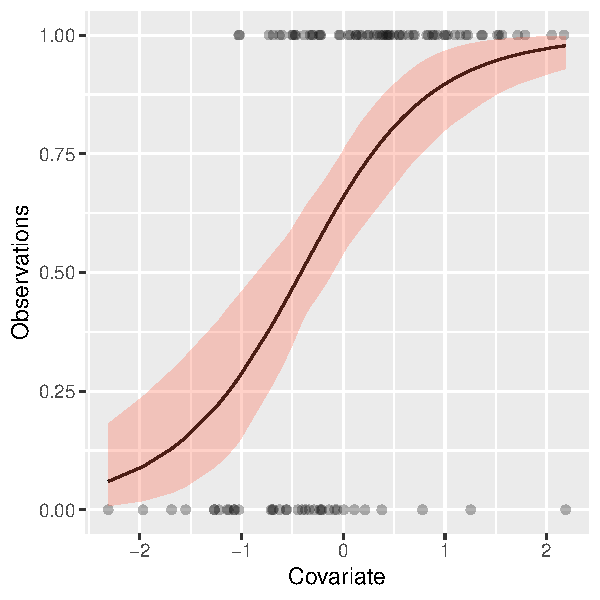
\includegraphics{day1_practical_files/figure-pdf/unnamed-chunk-52-1.pdf}
\end{center}

\end{tcolorbox}

\subsection{Generalised Additive Model}\label{sec-gam_ex}

In this practical we will:

\begin{itemize}
\tightlist
\item
  Learn how to fit a GAM with \texttt{inlabru}
\item
  Generate predictions from the model
\end{itemize}

Generalised Additive Models (GAMs) are very similar to linear models,
but with an additional basis set that provides flexibility.

Additive models are a general form of statistical model which allows us
to incorporate smooth functions alongside linear terms. A general
expression for the linear predictor of a GAM is given by

\[
\eta_i = g(\mu_i) = \beta_0 + \sum_{j=1}^L f_j(x_{ij}) 
\]

where the mean
\(\pmb{\mu} = E(\mathbf{y}|\mathbf{x}_1,\ldots,\mathbf{x}_L)\) and
\(g()\) is a link function (notice that the distribution of the response
and the link between the predictors and this distribution can be quite
general). The term \(f_j()\) is a smooth function for the \emph{j}-th
explanatory variable that can be represented as

\[
f(x_i) = \sum_{k=0}^q\beta_k b_k(x_i)
\]

where \(b_k\) denote the basis functions and \(\beta_K\) are their
coefficients.

Increasing the number of basis functions leads to a more \emph{wiggly}
line. Too few basis functions might make the line too smooth, too many
might lead to overfitting.To avoid this, we place further constraints on
the spline coefficients which leads to constrained optimization problem
where the objective function to be minimized is given by:

\[
\mathrm{min}\sum_i(y_i-f(x_i))^2 + \lambda(\sum_kb^2_k)
\] The first term measures how close the function \(f()\) is to the data
while the second term \(\lambda(\sum_kb^2_k)\), penalizes the roughness
in the function. Here, \(\lambda >0\) is known as the smoothing
parameter because it controls the degree of smoothing (i.e.~the
trade-off between the two terms). In a Bayesian setting,including the
penalty term is equivalent to setting a specific prior on the
coefficients of the covariates.

In this exercise we will set a random walk prior of order 1 on \(f\),
i.e.~\(f(x_i)-f(x_i-1) \sim \mathcal{N}(0,\sigma^2_f)\) where
\(\sigma_f^2\) is the smoothing parameter such that small values give
large smoothing. Notice that we will assume \(x_i\)'s are equally spaced
for now (we will cover a stochastic differential equation approach that
relaxes this assumption later on in the course).

\subsubsection{Simulate Data}\label{simulate-data}

Lets generate some data so evaluate how RW models perform when
estimating a smooth curve. The data are simulated from the following
model:

\[
y_i = 1 + \mathrm{cos}(x) + \epsilon_i, ~ \epsilon_i \sim \mathcal{N}(0,\sigma^2_\epsilon)
\] where \(\sigma_\epsilon^2 = 0.25\)

\begin{Shaded}
\begin{Highlighting}[]
\NormalTok{n }\OtherTok{=} \DecValTok{100}
\NormalTok{x }\OtherTok{=} \FunctionTok{rnorm}\NormalTok{(n)}
\NormalTok{eta }\OtherTok{=}\NormalTok{ (}\DecValTok{1} \SpecialCharTok{+} \FunctionTok{cos}\NormalTok{(x))}
\NormalTok{y }\OtherTok{=} \FunctionTok{rnorm}\NormalTok{(n, }\AttributeTok{mean =}\NormalTok{  eta, }\AttributeTok{sd =} \FloatTok{0.5}\NormalTok{)}

\NormalTok{df }\OtherTok{=} \FunctionTok{data.frame}\NormalTok{(}\AttributeTok{y =}\NormalTok{ y, }
                \AttributeTok{x\_smooth =} \FunctionTok{inla.group}\NormalTok{(x)) }\CommentTok{\# equidistant x\textquotesingle{}s }
\end{Highlighting}
\end{Shaded}

\subsubsection{\texorpdfstring{Fitting a GAM in
\texttt{inlabru}}{Fitting a GAM in inlabru}}\label{fitting-a-gam-in-inlabru}

Now lets fit a flexible model by setting a random walk of order 1 prior
on the coefficients. This can be done bye specifying
\texttt{model\ =\ "rw1"} in the model component (similarly,a random walk
of order 2 can be placed by setting \texttt{model\ =\ "rw2"} )

\begin{Shaded}
\begin{Highlighting}[]
\NormalTok{cmp }\OtherTok{=}  \ErrorTok{\textasciitilde{}} \FunctionTok{Intercept}\NormalTok{(}\DecValTok{1}\NormalTok{) }\SpecialCharTok{+} 
  \FunctionTok{smooth}\NormalTok{(x\_smooth, }\AttributeTok{model =} \StringTok{"rw1"}\NormalTok{)}
\end{Highlighting}
\end{Shaded}

Now we define the observational model:

\begin{Shaded}
\begin{Highlighting}[]
\NormalTok{lik }\OtherTok{=}  \FunctionTok{bru\_obs}\NormalTok{(}\AttributeTok{formula =}\NormalTok{ y }\SpecialCharTok{\textasciitilde{}}\NormalTok{.,}
            \AttributeTok{family =} \StringTok{"gaussian"}\NormalTok{,}
            \AttributeTok{data =}\NormalTok{ df)}
\end{Highlighting}
\end{Shaded}

We then can fit the model:

\begin{Shaded}
\begin{Highlighting}[]
\NormalTok{fit }\OtherTok{=} \FunctionTok{bru}\NormalTok{(cmp, lik)}
\NormalTok{fit}\SpecialCharTok{$}\NormalTok{summary.fixed}
\end{Highlighting}
\end{Shaded}

\begin{verbatim}
              mean         sd 0.025quant 0.5quant 0.975quant     mode      kld
Intercept 1.298799 0.06506722    1.17164 1.298565   1.427294 1.298569 158.5814
\end{verbatim}

The posterior summary regarding the estimated function using RW1 can be
accessed through \texttt{fit\$summary.random\$smooth}, the output
includes the value of \(x_i\) (\texttt{ID}) as well as the posterior
mean, standard deviation, quantiles and mode of each \(f(x_i)\). We can
use this information to plot the posterior mean and associated 95\%
credible intervals.

\section{R plot}

\begin{figure}[H]

{\centering 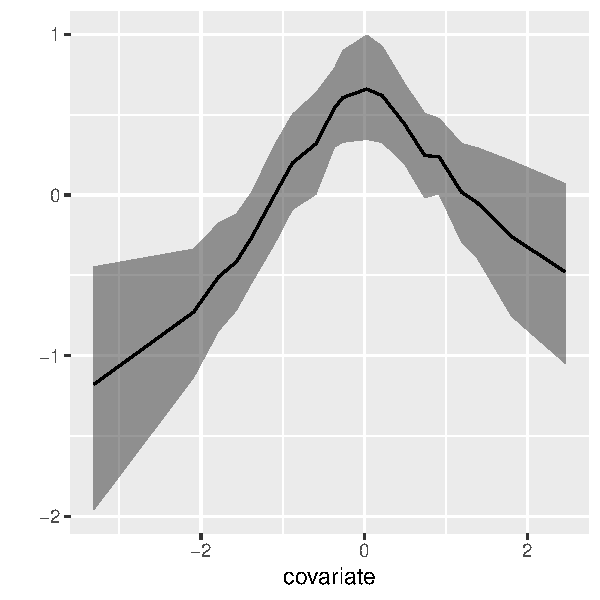
\includegraphics{day1_practical_files/figure-pdf/unnamed-chunk-68-1.pdf}

}

\caption{Smooth effect of the covariate}

\end{figure}%

\section{R Code}

\begin{Shaded}
\begin{Highlighting}[]
\FunctionTok{data.frame}\NormalTok{(fit}\SpecialCharTok{$}\NormalTok{summary.random}\SpecialCharTok{$}\NormalTok{smooth) }\SpecialCharTok{\%\textgreater{}\%} 
  \FunctionTok{ggplot}\NormalTok{() }\SpecialCharTok{+} 
  \FunctionTok{geom\_ribbon}\NormalTok{(}\FunctionTok{aes}\NormalTok{(ID,}\AttributeTok{ymin =}\NormalTok{ X0}\FloatTok{.025}\NormalTok{quant, }\AttributeTok{ymax=}\NormalTok{ X0}\FloatTok{.975}\NormalTok{quant), }\AttributeTok{alpha =} \FloatTok{0.5}\NormalTok{) }\SpecialCharTok{+} 
  \FunctionTok{geom\_line}\NormalTok{(}\FunctionTok{aes}\NormalTok{(ID,mean)) }\SpecialCharTok{+} 
  \FunctionTok{xlab}\NormalTok{(}\StringTok{"covariate"}\NormalTok{) }\SpecialCharTok{+} \FunctionTok{ylab}\NormalTok{(}\StringTok{""}\NormalTok{)}
\end{Highlighting}
\end{Shaded}

\subsubsection{Model Predictions}\label{model-predictions-1}

We can obtain the model predictions using the \texttt{predict} function.

\begin{Shaded}
\begin{Highlighting}[]
\NormalTok{pred }\OtherTok{=} \FunctionTok{predict}\NormalTok{(fit, df, }\SpecialCharTok{\textasciitilde{}}\NormalTok{ (Intercept }\SpecialCharTok{+}\NormalTok{ smooth))}
\end{Highlighting}
\end{Shaded}

The we can plot them together with the true curve and data points:

\begin{Shaded}
\begin{Highlighting}[]
\NormalTok{pred }\SpecialCharTok{\%\textgreater{}\%} \FunctionTok{ggplot}\NormalTok{() }\SpecialCharTok{+} 
  \FunctionTok{geom\_point}\NormalTok{(}\FunctionTok{aes}\NormalTok{(x\_smooth,y), }\AttributeTok{alpha =} \FloatTok{0.3}\NormalTok{) }\SpecialCharTok{+}
  \FunctionTok{geom\_line}\NormalTok{(}\FunctionTok{aes}\NormalTok{(x\_smooth,}\DecValTok{1}\SpecialCharTok{+}\FunctionTok{cos}\NormalTok{(x\_smooth)),}\AttributeTok{col=}\DecValTok{2}\NormalTok{)}\SpecialCharTok{+}
  \FunctionTok{geom\_line}\NormalTok{(}\FunctionTok{aes}\NormalTok{(x\_smooth,mean)) }\SpecialCharTok{+}
  \FunctionTok{geom\_line}\NormalTok{(}\FunctionTok{aes}\NormalTok{(x\_smooth, q0}\FloatTok{.025}\NormalTok{), }\AttributeTok{linetype =} \StringTok{"dashed"}\NormalTok{)}\SpecialCharTok{+}
  \FunctionTok{geom\_line}\NormalTok{(}\FunctionTok{aes}\NormalTok{(x\_smooth, q0}\FloatTok{.975}\NormalTok{), }\AttributeTok{linetype =} \StringTok{"dashed"}\NormalTok{)}\SpecialCharTok{+}
  \FunctionTok{xlab}\NormalTok{(}\StringTok{"Covariate"}\NormalTok{) }\SpecialCharTok{+} \FunctionTok{ylab}\NormalTok{(}\StringTok{"Observations"}\NormalTok{)}
\end{Highlighting}
\end{Shaded}

\begin{figure}[H]

{\centering 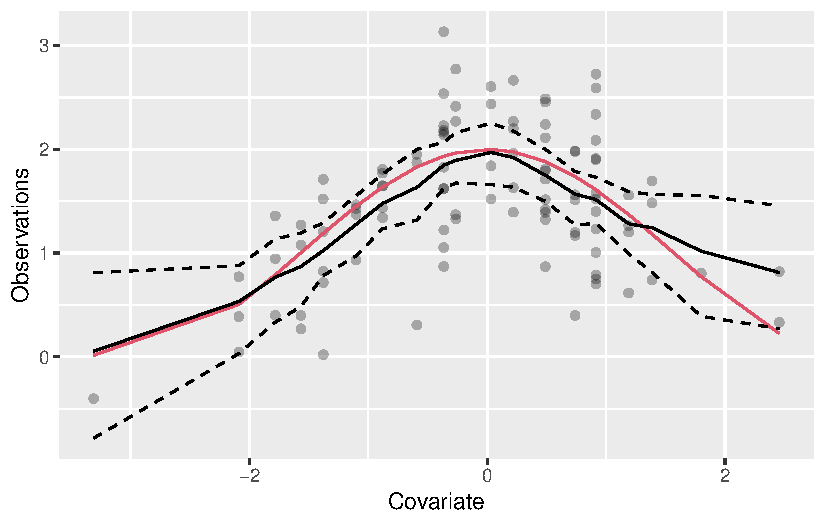
\includegraphics{day1_practical_files/figure-pdf/plot_gam-1.pdf}

}

\caption{Data and 95\% credible intervals}

\end{figure}%

\begin{tcolorbox}[enhanced jigsaw, toprule=.15mm, coltitle=black, opacitybacktitle=0.6, colframe=quarto-callout-warning-color-frame, breakable, colback=white, opacityback=0, leftrule=.75mm, arc=.35mm, rightrule=.15mm, bottomrule=.15mm, colbacktitle=quarto-callout-warning-color!10!white, title={Task}, toptitle=1mm, titlerule=0mm, left=2mm, bottomtitle=1mm]

Fit a flexible model using a random walk of order 2 (RW2) and compare
the results with the ones above.

Take hint

You can set \texttt{model\ =\ "rw2"} for assigning a random walk 2
prior.

Click here to see the solution

\begin{Shaded}
\begin{Highlighting}[]
\NormalTok{cmp\_rw2 }\OtherTok{=}  \ErrorTok{\textasciitilde{}} \FunctionTok{Intercept}\NormalTok{(}\DecValTok{1}\NormalTok{) }\SpecialCharTok{+} 
  \FunctionTok{smooth}\NormalTok{(x\_smooth, }\AttributeTok{model =} \StringTok{"rw2"}\NormalTok{)}
\NormalTok{lik\_rw2 }\OtherTok{=}  \FunctionTok{bru\_obs}\NormalTok{(}\AttributeTok{formula =}\NormalTok{ y }\SpecialCharTok{\textasciitilde{}}\NormalTok{.,}
            \AttributeTok{family =} \StringTok{"gaussian"}\NormalTok{,}
            \AttributeTok{data =}\NormalTok{ df)}
\NormalTok{fit\_rw2 }\OtherTok{=} \FunctionTok{bru}\NormalTok{(cmp\_rw2, lik\_rw2)}

\CommentTok{\# Plot the fitted functions}
\FunctionTok{ggplot}\NormalTok{() }\SpecialCharTok{+} 
  \FunctionTok{geom\_line}\NormalTok{(}\AttributeTok{data=}\NormalTok{ fit}\SpecialCharTok{$}\NormalTok{summary.random}\SpecialCharTok{$}\NormalTok{smooth,}\FunctionTok{aes}\NormalTok{(ID,mean,}\AttributeTok{colour=}\StringTok{"RW1"}\NormalTok{),}\AttributeTok{lty=}\DecValTok{2}\NormalTok{) }\SpecialCharTok{+} 
  \FunctionTok{geom\_line}\NormalTok{(}\AttributeTok{data=}\NormalTok{ fit\_rw2}\SpecialCharTok{$}\NormalTok{summary.random}\SpecialCharTok{$}\NormalTok{smooth,}\FunctionTok{aes}\NormalTok{(ID,mean,}\AttributeTok{colour=}\StringTok{"RW2"}\NormalTok{)) }\SpecialCharTok{+} 
  \FunctionTok{xlab}\NormalTok{(}\StringTok{"covariate"}\NormalTok{) }\SpecialCharTok{+} \FunctionTok{ylab}\NormalTok{(}\StringTok{""}\NormalTok{) }\SpecialCharTok{+} \FunctionTok{scale\_color\_discrete}\NormalTok{(}\AttributeTok{name=}\StringTok{"Model"}\NormalTok{)}
\end{Highlighting}
\end{Shaded}

\begin{center}
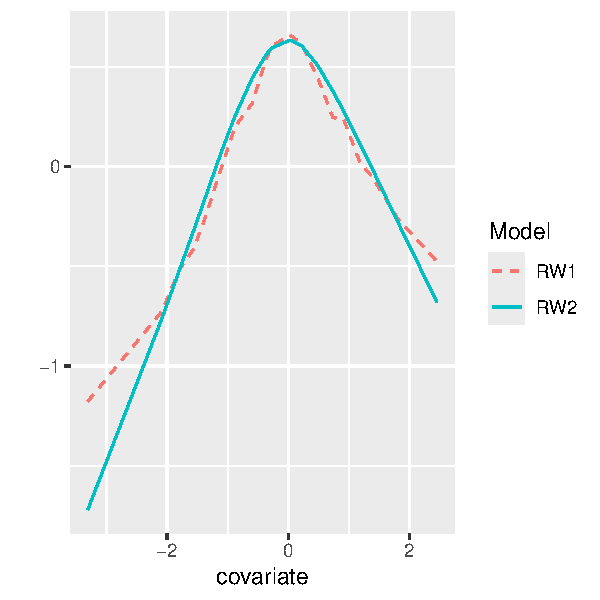
\includegraphics{day1_practical_files/figure-pdf/unnamed-chunk-70-1.pdf}
\end{center}

We see that the RW1 fit is too wiggly while the RW2 is smoother and
seems to have better fit.

\end{tcolorbox}



\end{document}
